\RequirePackage{plautopatch}
% \documentclass[report,paper=a4, fontsize=12pt, line_length=16cm, number_of_lines=33]{jlreq}
% \usepackage[haranoaji,deluxe]{luatexja-preset}
%\usepackage{amsmath,amssymb}
%\usepackage{libertinus}

\documentclass[report,paper=a4, fontsize=12pt, line_length=16cm, number_of_lines=33,dvipdfmx]{jlreq}
\usepackage{jlreq-deluxe}
\usepackage{amsmath,amssymb}
% \usepackage{libertine}
% \usepackage{libertinust1math}
% \usepackage[T1]{fontenc}
% \usepackage{mlmodern}
% \usepackage[T1]{fontenc}
% \usepackage{tgtermes,tgheros,tgcursor}
% \renewcommand{\bfdefault}{bx}
% \usepackage[libertine]{newtxmath}

%% Fonts
\usepackage{stix2}
%\usepackage{lmodern}
%\usepackage[T1]{fontenc}

\usepackage{hyperref}
\hypersetup{colorlinks=true,linkcolor=blue,citecolor=blue}

\usepackage{graphicx}
\graphicspath{{fig/}}

\usepackage{physics}
\usepackage{color}

\usepackage{tcolorbox}
\tcbuselibrary{breakable, skins, theorems}
%\usepackage{cleveref}

% font warningを出さないため
% \DeclareFontShape{JY2}{hgt}{b}{n}{<->ssub*hgt/bx/n}{}
% \DeclareFontShape{JY2}{hgt}{m}{it}{<->ssub*hgt/m/n}{}
% \DeclareFontShape{JT2}{hgt}{b}{n}{<->ssub*hgt/bx/n}{}
% \DeclareFontShape{JT2}{hgt}{m}{it}{<->ssub*hgt/m/n}{}

\newenvironment{myquote}{\begin{tcolorbox}[
  colback = blue!5, after = \noindent] }{\end{tcolorbox}}
\newenvironment{important}{\begin{tcolorbox}[
  colback = white,
  colframe = red!35,
  boxrule = 2mm,
  fonttitle = \bfseries,
  after = \noindent] }{\end{tcolorbox}}
\newenvironment{mycite}{\\ \qquad \textbullet\ }{\\}

\newtcolorbox{emphasize}[1][]{
  colback=orange!7,
  colframe=orange!80!red,
  coltitle=white,
  title={#1},
  fonttitle=\sffamily \bfseries, 
  sharp corners,
  boxrule=0.5mm
}
\newtcolorbox{proposition}[1][]{
  colback=white,
  colframe=green!40,
  coltitle=black,
  title={#1},
  fonttitle=\sffamily \bfseries, 
  sharp corners,
  boxrule=0.5mm
}

\newcommand{\qed}{■}
\newcommand{\kyou}[1]{{\sffamily \bfseries #1}}

\numberwithin{equation}{chapter}
%%%%%%%%%%%%%%%%%%%%%%%%%%%%%%%%%%%%%%%%%%%%%%%%%%%%%%%%%%%%%%%%%%%%%%
%                          often used macro
\newcommand{\del}{\partial}
\newcommand{\Cb}{\mathbb{C}}
\newcommand{\Zb}{\mathbb{Z}}
\newcommand{\CP}{\Cb \mathrm{P}}
%\newcommand{\strong}[1]{{\sffamily \gtfamily \bfseries #1}}
\newcommand{\Ztwo}{\mbox{$\mathbb{Z}_{2}$}}
\newcommand{\Hh}{\widehat{H}}
\newcommand{\Uh}{\widehat{U}}
\newcommand{\Vh}{\widehat{V}}
\newcommand{\Jh}{\widehat{J}}
\newcommand{\Qh}{\widehat{Q}}
\newcommand{\Oh}{\widehat{\mathcal{O}}}

\newcommand{\Ocal}{\mathcal{O}}
\newcommand{\Ocalh}{\widehat{\mathcal{O}}}
\newcommand{\U}{\mbox{U}}

\title{一般化対称性について}
\author{山口 哲}
\date{\today}
\begin{document}
\maketitle
\tableofcontents

\section*{まえがき}

このノートは2023年10月に東京大学駒場で行った集中講義のノートです。集中講義の機会をくださり、有益な議論をしてくださった東京大学駒場素粒子論研究室の皆様、集中講義の参加者の皆様に感謝いたします。

\chapter{導入}
\section{対称性とは?}

この講義では、対称性の一般化について取り扱います。一般化に行くまえに普通の対称性について質問したいと思います。(場の理論において)対称性とは何でしょうか?考えてみてください。この質問は哲学的に聞こえるかもしれませんが、もっと具体的なもので、例えばみなさんが授業や教科書でどう習ったか、あるいは授業どう教えているかというものです。

答えはいろいろあると思います。ここでは、その中の3つをとりあえず書いてみます。この中に皆さんの考えた答えはあるでしょうか?
\begin{itemize}
  \item[①] 場を$\phi$、作用を$S(\phi)$とします。対称性とは変換$\phi\to\phi'$であって$S(\phi')=S(\phi)$となるものです。
  \item[②] Hamiltonianを$\Hh$とします。対称性とはUnitary演算子$\Uh$であって、Hamiltonianと交換する、つまり$\Hh \Uh =\Uh \Hh$となるものです。
  \item[③] 余次元1のトポロジカル欠陥で群構造を持つもの。  
\end{itemize}
①は、一番人気がある答えで、多くの人がこれを思い浮かべたと思います。②も量子力学では良く出てくる説明で、これを思い浮かべなかった人も言われてみれば納得してもらえると思います。③は異質ですね。これは普通の教科書には載っていないです。意味が分からなかったとしてもひとまず気にしないでください。③はこの後この講義で時間をかけて説明したいことの一つです。これが①や②と同じレベルで納得してもらえれば、この講義の目的の目的の半分くらいは達成したと言えます。

さて、①や②のような分かりやすい言い方があるのに、なぜ③のような難しい言い方を知らないといけないのでしょうか。実は①や②には次のように「大域的である」という共通の不満があるのです。
\begin{itemize}
  \item[①] 変換は時空全体で一斉に変換してみることが必要になります。宇宙を考えているなら、宇宙の始まりから未来まで、ほぼ真空のところや星の中から宇宙の果てまで一斉に変換して作用が不変か?という問でしか対称性の存在を記述できていません。
  \item[②] こちらは時間方向は考えなくても良いですが、$\Hh$も$\Uh$も空間全体に広がる巨大な演算子です。しかも系のサイズによって(Hilbert空間の次元も含めて)変わります。 両方とも局所的なものの集まりなので、局所的な性質を見れば全体をいっぺんに考えなくても良いはずなのですが、②の言い方では全体でしか考えられていません。
\end{itemize}
つまり、対称性の記述としては
\begin{emphasize}
  (大域的対称性であっても)局所的な記述が望ましい。
\end{emphasize}
ということになります。

この不満は最近になって降って湧いたわけではなく、昔からありました。そしてその解決もされています。それが、最初の質問に対する4番目の答えです。
\begin{itemize}
  \item[④] 対称性とは、(連続対称性の無限小変換の場合には)カレント$J^{\mu}(x)$であって、$\del_{\mu}J^{\mu}(x)=0$を満たすことである。
\end{itemize}
最初の問でこれを思い浮かべられた方もおられたかも知れません。また、言われてみれば皆さん納得されると思います。この記述は完全に局所的で理想通りです。場の理論で対称性を用いて様々な性質を導くときに、この記述は大変便利で、欠くことができないものです。

④の答えは非常に良いものでしたが、難点は連続対称性の無限小変換に限られることです。例えば離散的対称性の場合にはカレントは存在しませんから、④の記述はありません。実は離散的な対称性の場合にも適用できる局所的な記述が③です。
\begin{emphasize}
  ③のトポロジカル欠陥は対称性の局所的な記述を与える。  
\end{emphasize}
このような理由で③の見方は、普通の対称性に対しても有用です。

\section{対称性の使い方の例}

この後、対称性の一般化について説明していくわけですが、対称性を一般化しても有用であるということを説明するために、対称性の使い方の一つをについて説明します。これは簡単な例ですが、量子力学の教科書にはあまり書いてないと思います。

次のような命題が成り立ちます。
\begin{proposition}[命題]
$\Uh,\Vh$をユニタリー演算子で、Hamiltonian $\Hh$と可換とします(つまり、②の見方での対称性です。)。そして
\begin{align}
  \Uh \Vh = a \Vh \Uh,\quad (a \text{はc数},\ a\ne 1)
  \label{anomaly}
\end{align}  
とします。このとき、\kyou{すべてのエネルギー準位(特に基底状態)は縮退しています。}
\end{proposition}
これは、場の理論の文脈では 't Hooft アノマリー整合条件と呼ばれているものの一例です。$a$がこの例での 't Hooft アノマリーになります。おそらく、普通に場の理論でアノマリーを勉強された方には、そのアノマリーとこの$a$がどう関係があるか分からないと思います。大事なことではあるのですが、この講義の主題とは外れるのと、知らなくてもこの命題だけで理解できるので、その説明は省略します。

\kyou{証明} 証明を与えます。背理法で証明します。つまり、縮退していないエネルギー固有状態$\ket{\psi},\ \Hh \ket{\psi}=E\ket{\psi}$があると仮定します。このとき$\Uh\ket{\psi}$がエネルギー$E$の固有状態であることが、次のようにして分かります。
\begin{align}
  \Hh \Uh \ket{\psi} =\Uh \Hh \ket{\psi}
  =E\Uh \ket{\psi}.
\end{align}
さらに縮退が無いことがら$\Uh \ket{\psi}\propto \ket{\psi}$なので、次のように表すことができます。
\begin{align}
  \Uh \ket{\psi}=u\ket{\psi},\ u\in \Cb,\ |u|=1.
\end{align}
$\Vh$に関しても同様です。
\begin{align}
  \Vh \ket{\psi}=v\ket{\psi},\ v \in \Cb,\ |v|=1.
\end{align}
これらを用いると
\begin{align}
  \Uh \Vh \ket{\psi}=uv\ket{\psi}
\end{align}
という関係を得ます。ところが、\eqref{anomaly}の関係を用いると、全く同じベクトルが
\begin{align}
  \Uh \Vh \ket{\psi}=a\Vh \Uh \ket{\psi}=a u v \ket{\psi}
\end{align}
とも書けます。ここから
\begin{align}
  auv\ket{\psi}=uv\ket{\psi}
\end{align}
という関係式を得ます。$uv\ket{\psi}\ne 0$ですから、この式は$a\ne 1$に矛盾します。\qed 

ここで考えてみたいことは、\kyou{$\Uh,\Vh$ がユニタリーでなかったらどうなるか?}ということです。この場合、$\Uh,\Vh$ ユニタリーではありませんから、従来の意味での対称性ではありません。しかし、証明を見てもらって分かるように、ユニタリー性を用いているところは$uv\ket{\psi}\ne 0$の部分のみです。ですから、この場合も命題を少し修正することで成り立ちます。このようにして「(従来の意味では)対称性でないもの」を対称性と同じように用いて理論を調べることができるわけです。このように従来の意味では対称性でないが、対称性と同様な使い方ができるものを「一般化対称性」と呼んでいろいろ調べようというのがここでやりたいことです。

上の証明を見てもらって分かるように、対称性の最も重要な性質はHamiltonianと交換するということです。これをゆるめてしまうと、対称性と同じように用いることは、なかなか難しくなります。したがって、ここではこの条件はゆるめないことにします。一方、ユニタリーのような条件はゆるめても、そこそこ使えるものになります。これを「一般化対称性」と呼んで、いろいろ調べよう、というのがこの講義の目的です。ユニタリーでないがHamiltonianと交換する演算子は場の理論の文脈では「非可逆対称性」と呼ばれます。\footnote{非可逆対称性という名前の由来については、少々複雑です。ちゃんと説明するためには場の理論でのトポロジカル欠陥について知ってもらう必要があります。ここでは、\kyou{非可逆対称性という名前だけれど$\Uh$という演算子が非可逆とは限らない}、ということだけ注意しておきます。}

\section{いくつかの注意}\label{sec:remarks}
ここでは、通常のセミナーなどでは説明が省略されることが多いけれど、注意が必要なことについて説明します。

一つは、Euclideanの定式化についてです。この講義も含めて、セミナーや論文などでは場の理論をEuclid形式で取り扱うことがよくあります。これは、「Euclid形式の場の理論」という、教科書に出てくる場の理論と異なる理論を考えているのではないことに注意してください。理論は教科書に出てくる場の理論と同じものを取り扱っています。異なるのは定式化の仕方とか計算しやすい量です。例えば正準分配関数はEuclid形式で取り扱いやすい量の一つです。これは
\begin{align}
  \Tr e^{-\beta \Hh} = \int D\phi e^{-S_{E}(\phi)}
\end{align}
のように表すことができます。ここで、$S_{E}(\phi)$は虚時間方向を長さ$\beta$の円周にしたときのEuclid化した作用です。他にも、$\Ocalh_1(x_1),\dots, \Ocalh_K(x_K)$をすべて同時刻の別々の点に置かれた局所演算子としたとき、
\begin{align}
  \expval{\Ocalh_1(x_1) \dots \Ocalh_K(x_K)}{0}
  =\frac{1}{Z}\int D\phi e^{-S_{E}(\phi)} \Ocal_1(x_1) \dots \Ocal_K(x_K),\quad 
  Z:=\int D\phi e^{-S_{E}(\phi)}.
\end{align}
と表すことができます。このとき$S_E(\phi)$はEuclid化した作用です。他にも様々な量がEuclid形式を用いて計算することができます。この講義でもEuclid形式用いて様々な場の理論の性質を考えることになります。

もう一つは演算子関係式についてです。例えば、この講義でも\kyou{量子論で}
\begin{align}
  \del_{\mu}J^{\mu}(x)=0\label{egoperatorrelation}
\end{align}
というような式を書くことがあります。これは古典論であれば、運動方程式を満たす場の配位において、このような関係式を満たすということですが、量子論においてはどうでしょうか?一つは演算子形式の場の理論で$\Jh^\mu(x)$が上の関係式を満たすということです。この講義で主に用いるのは、もう少し広い応用ができる見方で、相関関数の間の関係式と見ることです。これは、
\begin{align}
  \expval{\del_{\mu}J^{\mu}(x)\cdots}=0,&\quad(\text{$\cdots$は任意の局所演算子や非局所演算子の挿入。}\notag\\&\text{ただし$x$は$\cdots$の挿入されている点とは異なる。})
\end{align}
というのを省略して書いたのが式\eqref{egoperatorrelation}ということです。問題は「ただし…」のところは文脈によって色々変わるところです。この講義では分かりにくそうな場合はなるべく補足するようにはしますが、もし分からなければ聞いてください。

他によく使う例として
\begin{align}
  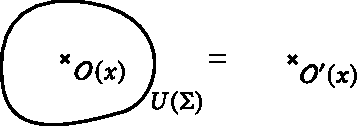
\includegraphics{EgWTid.pdf}
\end{align}
というようなものがあります。これは$x$は時空の点で$\Ocal(x),\Ocal'(x)$は局所演算子、$\Sigma$はcodimension 1の面で$U(\Sigma)$は$\Sigma$に局在した演算子(欠陥)です。この「式」の意味は
\begin{align}
  \expval{U(\Sigma)\Ocal(x)\cdots}=\expval{\Ocal'(x)\cdots},\qquad&(\text{$\cdots$は両辺で共通の任意の演算子の挿入。 }\notag \\
  &\text{ただし、$\cdots$は$\Sigma$の内側には挿入されていない。})
\end{align}
という意味です。

\chapter{対称性とトポロジカル欠陥}

この章の目標は、前章で紹介した対称性の③の見方「対称性とは余次元1のトポロジカル欠陥で群構造を持つもの」ということを納得してもらうことです。まず、欠陥という概念を導入します。そして対称性がトポロジカル欠陥であることを様々な観点から説明します。一旦それを納得してもらえば、対称性の一般化はすんなりと納得してもらえると思います。

\section{欠陥}

まず、欠陥を定義します。
\begin{emphasize}
  場の理論において\kyou{欠陥(defect)}とは、\kyou{時空の中で他の部分と性質が異なる部分}のことを言います。 ただし、局所性を満たすものとします。 
\end{emphasize}

補足の説明をします。性質が異なるというのは、例えばLagrangian密度がそこだけ異なるとか、余分な自由度がそこにあるとか、格子の理論なら、そこだけ格子の構造が異なるとか、そういうものです。

局所性というのは、性質が異なるとしても非局所的な相互作用はないということです。言い換えれば、欠陥の上の離れた2点が直接相互作用をすることは無いようなものです。格子理論で考える場合には、連続極限をとったときに局所性を満たすようなものなら、それは局所性を満たす欠陥であると言うことにします。

別の言い方をすると、欠陥とは(広い意味での)演算子であるということもできます。

次に2つの言葉を導入します。まず、欠陥の\kyou{次元}とは、性質の異なる部分の次元を言います。例えば時空の中で1点が他の部分と異なるなら、その次元は1です。\kyou{余次元(codimension)}とは、時空の次元を$d$、欠陥の次元を$p$としたときに、$d-p$のことを言います。欠陥の性質は余次元によって共通な場合もあるので、この言葉を導入するのが便利です。これは単に言葉遣いの問題なのですが、余次元0の欠陥、つまりある領域にわたって性質が違うようなものは欠陥とは呼ばないことにします。

代表的な欠陥の例を2つ挙げます。局所演算子は0次元の欠陥です。別の言い方をするなら、局所演算子とは時空の1点にある欠陥の別名です。\footnote{局所演算子はLagrangianに出てくる場の微分やそれらの積で書けているものに限りません。}もう一つの例はゲージ理論のWilsonループ$\Tr P \exp\left(i\oint A\right)$です。Wilsonループは1次元の欠陥の例です。

欠陥について一つ注意することは、欠陥は動的な物体、例えばソリトンなどではないということです。動的な物体は運動方程式などにしたがって運動しますが、欠陥はその部分の物理法則を手で変えるようなものです。欠陥の形などは手で決めます。ややこしいことに文献によってはソリトンのことを欠陥と呼んでいるものもあるので注意が必要です。

\section{対称性とトポロジカル欠陥その1}

ここから対称性とトポロジカル欠陥の関係について見ていきます。

まず、\kyou{トポロジカル欠陥(topological defect)}とは、欠陥のうちでトポロジーを変えない連続変形で値を変えないもののことを言います。\footnote{これも不幸な用語の行き違いなのですが、トポロジー的に守られて安定なソリトンのことをトポロジカル欠陥と呼ぶ文献もあります。これはこの講義でのトポロジカル欠陥とは違うものです。}
絵を使った式で書くなら
\begin{align}
  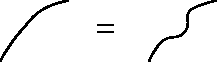
\includegraphics{topologicaldefect.pdf}
\end{align}
のようになります。この式も\ref{sec:remarks}節で述べた演算子関係式の書き方を使っています。つまり、左辺と右辺は他に任意の共通の演算子が挿入されている期待値です。ただし、欠陥を変形している部分には演算子は挿入されていません。

ここから考えていきたいことは、みなさんが納得しているはずの対称性の見方②$\Hh \Uh = \Uh \Hh$、および④$\del_{\mu}J^{\mu}=0$から始めて、③トポロジカル欠陥の見方ができることを示すことです。

\subsection{ユニタリー演算子とトポロジカル欠陥}

$d$次元の場の理論の演算子形式の定式化から始めることにします。簡単のために$\U (1)$対称性の場合を考えます。時刻$0$で対称性のユニタリー演算子は変換のパラメーターを$\alpha$として、
\begin{align}
  \Uh=e^{i\alpha \Qh},\qquad
  \Qh:=\int_{t=0,\ \text{空間}}d^{d-1}x \Jh^0. 
\end{align}
$\Jh^{0}$はカレント$\Jh^{\mu},\ \mu=0,\dots,d-1$の時間方向成分、つまり電荷密度です。$\Qh$の定義は空間が有限(周期境界条件など)の場合には良いですが、無限の場合には積分が定義されるかどうかが問題となります。実は自発的対称性の破れが起こっている場合には、この積分は収束しません。自発的対称性の破れについては、教科書\cite{Kugo2}が詳しいです。ここではひとまず定義されている場合を考えることにします。

Euclideanの定式化を使うために、
\begin{align}
  \Jh^{d}:=i\Jh^{0}
\end{align}
を定義します。\footnote{これを見て分かるように、Euclideanの定式化ではHermit共役には注意する必要があります。} これを用いると
\begin{align}
  \Qh = -i \int_{t=0,\ \text{空間}}d^{d-1}x \Jh^{d}
\end{align}
と書けます。

Euclid時間(虚時間)を$\tau$として、Euclid時間発展について考えます。$\Oh$を時刻$0$での演算子として、Heisenberg演算子のような役割をする演算子$\Oh(\tau)$を
\begin{align}
  \Oh(\tau):=e^{\tau \Hh}\Oh e^{-\tau \Hh}
\end{align}
と定義します。\footnote{本当のHeisenberg演算子と区別するために記号を変える方が良いのかもしれませんが、煩雑になるのでやめておきます。本物のHeisenberg演算子とは違うものであることに注意してください。また、ここで定義したEuclideanのHeisenberg演算子のようなものは取り扱いには注意が必要です。$e^{|\tau| \Hh}$という高エネルギーのところが大きく効いてくる演算子が入っているからです。ただし、これらの演算子の時間順序積の真空期待値などはちゃんと定義されます。Euclideanの経路積分形式と演算子形式をつなぐときに考えると便利な書き方だと思うと良いと思います。} こうすると、例えばカレントの保存則$\del_{\mu}\Jh^{\mu}(x^0,\vec{x})=0,\ \mu=0,\dots, d-1$は、$x^d:=\tau$として
\begin{align}
  \del_{\mu}\Jh^{\mu}(\vec{x},x^{d})=0,\ \mu=1,\dots,d
\end{align}
と書くことができます。また、$\Uh \Hh = \Hh \Uh$ですから
\begin{align}
  \Uh(\tau)=\Uh
  \label{conservation}
\end{align}
となります。

式\eqref{conservation}をEuclidean経路積分形式での期待値の関係式に書くと
\begin{align}
  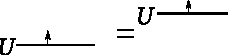
\includegraphics{conservation.pdf}\label{coservationfig}
\end{align}
のようになります。ここで矢印で向きを表しています。

$U$は時間一定面で他の部分とは異なっているので、余次元1の欠陥です。式\eqref{coservationfig}は、$U$を時間方向にずらしても値を変えないことを示しています。これから、$U$がトポロジカル欠陥であることを示します。

これから書くのはEuclidean経路積分形式での演算子関係式です。余次元1の向きのついた部分多様体を$M$として
\begin{align}
  U(M):=e^{i\alpha \Qh(M)},\quad
  Q(M):=-i\int_{M}dS_{\mu}J^{\mu}
\end{align}
とします。\footnote{$U(M)$の定義の中に$\exp$があって、同じ点での演算子の積が入っています。一般には、ここで発散があったり、繰り込みが必要だったりして微妙なことが起こるのですが、ここではひとまず説明のために無視します。正しい取り扱いは、次節でやる背景ゲージ場とそのゲージ変換を用いる方法です。}$\int_{M}dS_{\mu}$は電磁気の授業などで出てきた面積分です。

この$U(M)$がトポロジカルであることは次のようにして示します。ある領域$D$があって、$\del D=M\cup (-M')$とします。ただし、$-M'$は$M'$の向きを反対にしたものです。こうするとGaussの定理を用いて
\begin{align}
  \int_{D}d^d x \del_{\mu}J^{\mu}
  =\int_{M}dS_{\mu}J^{\mu}-\int_{M'}dS_{\mu}J^{\mu}
\end{align}
を得ます。ここから
\begin{align}
  Q(M)=Q(M'),\qquad U(M)=U(M')
\end{align}
という式が成り立ちます。特に$M_1$と$M_2$がトポロジーを変えない連続変形で繋がっている場合には領域$D$で、$\del D=M_1\cup (-M_2)$となるものがとれますから、$U(M_1)=U(M_2)$となり、したがって$U$はトポロジカル欠陥ということが言えました。

ここまでで言えたことをまとめます。
\begin{emphasize}
  対称性があると対応するトポロジカル欠陥がある。それは、対称性の演算子$\Uh$を時間一定面だけでなく、曲がったところにも定義したものである。
\end{emphasize}
最初の方で、自発的対称性の破れがあるときには$\Uh$がうまく定義できないと言いました。しかし、これは定義しようとしている空間が無限であるところからくるものです。したがって、$M$が有限である場合には$U(M)$は自発的対称性の破れがあるかどうかにかかわらず定義でき、理論の解析に用いることができます。

\subsection{局所演算子への作用}

次に対称性の局所演算子への作用について考えてみます。場の理論の演算子形式では、局所演算子$\Oh(x)$変換は
\begin{align}
  \Uh \Oh(x) \Uh^{\dag}=\Oh'(x)
  \label{transformation0}
\end{align}
と書けます。\footnote{量子力学の教科書とは異なるconventionを用いています。場の理論の論文では、ここで用いるconventionの方が一般的です。}
$\Uh,\Uh^{\dag}$は$\Hh$と可換ですから、$\Uh$を少しだけ虚時間で未来に移動し、$\Uh^{\dag}$を少しだけ過去に移動することで
\begin{align}
  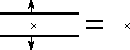
\includegraphics{transformation0.pdf}
\end{align}
という絵で表すことができます。別の言い方をすると式\eqref{transformation0}の左辺は、
\begin{align}
  T(\Uh(M_1)\Oh(x)\Uh(M_2))=T(\Uh(M)\Oh(x)),\quad
  M:=M_1 \cup (-M_2)
\end{align}
と表すことができます。$T()$は虚時間順序積を表します。さらに$\cdots$を$x$と同時刻にはない任意の演算子の挿入として\eqref{transformation0}より
\begin{align}
  \ev{T(\Uh(M)\Oh(x)\cdots)}{0}=\ev{T(\Oh'(x)\cdots)}{0}
\end{align}
という式が成り立ちます。この両辺に現れる量をEuclidean経路積分で表すことを想定して
\begin{align}
  \expval{U(M)\Ocal(x)\cdots}=\expval{\Ocal'(x)\cdots}
\end{align}
と書くのでした。さらにこれを略記して
\begin{align}
  U(M)\Ocal(x) = \Ocal'(x)
\end{align}
と書きます。$U(M)$はトポロジカルですから、連続変形して(変形後の面も同じ記号$M$で表すことにして)
\begin{align}
  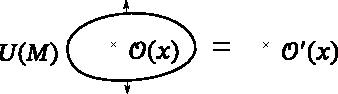
\includegraphics{transformation1.pdf}
\end{align}
という絵で書きます。これが、局所演算子の変換性をトポロジカル欠陥を用いて表したものになります。後で示すように、これはWard-Takahashi恒等式を有限変換の場合にも適用できる形にしたものと言うこともできます。

\section{対称性とトポロジカル欠陥その2}
ここでは、対称性とトポロジカル欠陥の関係を先程とは少し別の角度から見てみます。ここでは、通常のWard-Takahashi恒等式を①の描像から導くのと同様の方法を離散対称性の場合にも適用できるように有限変換で行います。つまり、大域的対称性であっても場所に依存する変換し、それによる作用の変化を見ます。

\subsection{分配関数と対称性欠陥}
$d$次元の場の理論を考えます。場を$\phi(x)$とし、作用を$S(\phi)$とします。この系に①の意味での大域的対称性があるとします。つまり、群$G$があり、$g\in G$に対して変換$\phi(x) \to \phi^g(x)$があって、$S(\phi^g)=S(\phi)$となるとします。$G$は連続的でも離散的でも良いです。

アイデアは、大域的対称性であっても場所に依存する変換、つまりゲージ変換をしてみることです。離散対称性でも適用できるように次のような変換を考えます。Euclidean時空の中の領域$D$をとり、変換
\begin{align}
  \phi'(x)=
  \begin{cases}
    \phi^g(x), & x\in D\\
    \phi(x), & x \notin D
  \end{cases}
  .\label{gaugetransf}
\end{align}
を考えます。つまり、領域$D$内では、$g$での変換を行い、$D$の外では変換しません。この変換を用いて分配関数を変形していきます。
\begin{align}
  Z&=\int D\phi e^{-S(\phi)}\notag\\
   &= \int D\phi' e^{-S(\phi')}\notag\\ 
   &= \int D\phi e^{-S_{D,g}(\phi)}.\label{derWT1}
\end{align}
この変形では、1行目から2行目は単に積分変数の文字を変えただけです。2行目から3行目へは変換\eqref{gaugetransf}を代入しました。簡単のため、この変換で積分測度$\int D\phi$は不変であることを仮定しました。また、$S_{D,g}(\phi):=S(\phi')$と定義しました。

さて、一般には変換で$S_{D,g}(\phi)\ne S(\phi)$です。どれくらい異なるかを考えてみましょう。まず、$D$の外部では$\phi(x)=\phi'(x)$ですから、同じです。一方、$D$の内部では$\phi\to \phi^g$が大域的対称性であることから、同じになることが分かります。つまり、\kyou{$S_{D,g}(\phi)$と$S(\phi)$は$M:=\del D$の部分でのみ異なることになります。} ですので、$M$に局在している演算子(欠陥)を
\begin{align}
  U_{g^{-1}}(M):=\exp(S(\phi)-S_{D,g}(\phi))
\end{align}
の挿入で定義することにします。すると\eqref{derWT1}から
\begin{align}
  Z=\int D\phi e^{-S(\phi)}U_{g^{-1}}(M)
\end{align}
を得ます。この両辺を$Z$で割ると
\begin{align}
  \expval{U_{g^{-1}}(M)}=1
\end{align}
という恒等式を得ます。これがWard-Takahashi恒等式の一種です。

$D$の外側に他の演算子(欠陥)がささっている場合も全く同様の変形ができて、次の恒等式を得ます。
\begin{align}
  \expval{U_{g^{-1}}(M)\cdots}=\expval{\cdots}
\end{align}
このような式を単に
\begin{align}
  U_{g^{-1}}(M)=1\quad (\text{ただし$M$の内側には他の演算子がささっていない})
\end{align}
と式で表したり、
\begin{align}
  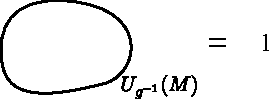
\includegraphics{EgWTid0.pdf}
\end{align}
と絵で表したりするのでした。

\subsection{演算子への作用}
この味方で演算子への作用を考えてみます。$\Ocal(x)$を局所演算子とし、それが$g\in G$で$\Ocal^{g}(x)$と変換するとします。

$D$の内部に$\Ocal(x)$を置き、その他の任意の演算子(欠陥)を$D$の外部に置きます。そして先程と同じように\eqref{gaugetransf}を考えます。すると
\begin{align}
  Z\expval{\Ocal(x)\cdots}
  =\int D\phi \Ocal(x)\cdots e^{-S(\phi)}
  =\int D\phi U_{g^{-1}}(M)\Ocal^{g}(x)\cdots e^{-S(\phi)}
\end{align}
という恒等式を得ます。これは
\begin{align}
  U_{g^{-1}}(M)\Ocal^{g}(x)=\Ocal(x)
\end{align}
と書くのでした。ここで、$\Ocal^{g}(x)$のことを$\Ocal(x)$と書き$g$のことを$g^{-1}$と書くことで
\begin{align}
  U_{g}(M)\Ocal(x)=\Ocal^{g}(x)
\end{align}
という恒等式を得ます。これは絵で
\begin{align}
  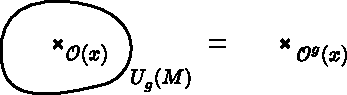
\includegraphics{EgWTid1.pdf}
\end{align}
というふうに表すこともできます。

$G$は群ですから、演算子への作用も表現になっています。ですから、表現行列を用いてWard-Takahashi恒等式を表しておくことも便利です。すべての局所演算子の基底を$\Ocal_{a}(x)$とすると、$\Ocal_{a}^{g}(x)$はこれらの線形結合で表すことができます。つまり$R(g)^{b}{}_{a}$を表現行列として
\begin{align}
  \Ocal^{g}_{a}(x)=\sum_{b}\Ocal_{b}(x)R(g)^{b}{}_{a}
\end{align}
と書くことができます。
これらすべてまとめて次のように言うことができます。
\begin{emphasize}
  離散的な群の場合も含めて、トポロジカル欠陥が対称性の局所的な記述を与える。この対称性を記述するトポロジカル欠陥を\kyou{対称性欠陥}と呼ぶ。Ward-Takahashi恒等式は
  \begin{align}
    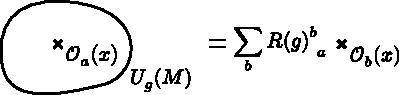
\includegraphics{EgWTid2.pdf}
  \end{align}
  と表せる。    
\end{emphasize}

\subsection{背景ゲージ場}
対称性を表すトポロジカル欠陥の便利な見方の一つは、背景ゲージ場を考えることです。結論から言うと、flatな背景ゲージ場の背景が対称性のトポロジカル欠陥の配位と同一視できます。それをこれから説明していきます。

簡単のため、連続対称性でアノマリーが無い場合を考えます。前節と同じ設定で、大域的対称性の背景ゲージ場$A$を入れた作用を$S(\phi,A)$とします。$A=0$のときに元の作用に戻るとします。つまり$S(\phi,A=0)=S(\phi)$とします。この背景ゲージ場の元での分配関数は
\begin{align}
  Z(A)=\int D\phi e^{-S(\phi,A)}
\end{align}
と表すことができます。

ここでゲージ変換について考えてみます。$A=0$のところから、前項で考えたゲージ変換\eqref{gaugetransf}をしてみます。このとき、$A\to A'$と変化します。ゲージ不変性は仮定しているので
\begin{align}
  Z(A=0)=Z(A')
\end{align}
となります。前項で議論したように、左辺は$M=\del D$に対称性欠陥が入った分配関数です。これがゲージ場$A'$が入っているのと同じということです。

$A'$は$A=0$から\eqref{gaugetransf}から得られたものですから、$A'$は$M$上だけでデルタ関数的に非0の値を持っています(図\ref{fig:localizedgaugefield}参照)。その値は$D$の中の点から外の点への経路で$M$と1回交わる経路を$C$として
\begin{align}
  P e^{i\int_{C}A'} = g
\end{align}
となるようになっています。また、もともと場の強さは$0$でしたから、ゲージ変換した後も$0$となります。このように場の強さが0となるゲージ場の配位を\kyou{flat}なゲージ場といいます。

\begin{figure}
  \centering
  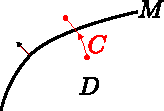
\includegraphics[width=6cm]{localizedgaugefield.pdf}
  \caption{対称性欠陥と背景ゲージ場の配位。$M$上にある対称性欠陥は$M$上にデルタ関数的に局在した背景ゲージ場の配位として表すことができる。$P e^{i\int_{C}A'} = g$ となるようになっている。}
  \label{fig:localizedgaugefield}
\end{figure}

この結果をまとめると
\begin{emphasize}
  対称性欠陥は、デルタ関数的に局在した背景ゲージ場の配位である。
\end{emphasize}
と言えます。

この逆を考えてみましょう。flatな背景ゲージ場の配位が与えられたとします。するとある点のまわりの球体のトポロジーを持つ領域でゲージ変換して、$A=0$とすることができます。これを図\ref{fig:localizedgaugefield}のように空間のいろんな部分からやっていって、ほとんどの部分で$A=0$とすることができます。しかし、二人の人が別の点からゲージ変換していって、ぶつかったときに、その間ですべて$A=0$とすることができるとは限りません。いっぱんに2つの領域の境目で$A\ne 0$となります。言い換えると、2つの領域の境目が対称性欠陥となります。

\begin{figure}
  \centering
  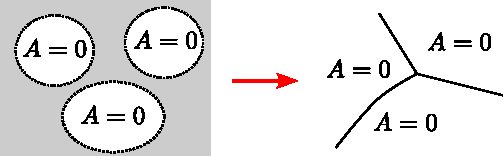
\includegraphics{flatgaugefield.pdf}
  \caption{flatな背景ゲージ場の配位と対称性欠陥の関係。右のようにいろんな点のまわりの球体の領域でゲージ変換を行って$A=0$となるようにする。領域の境目のみで$A\ne 0$になるが、これが対称性欠陥になる。}
  \label{fig:flatgaugefield}
\end{figure}

図\ref{fig:flatgaugefield}を見てもらっても分かるように、この操作を行うと一般的に対称性欠陥が枝分かれしている\kyou{ジャンクション}ができます。ゲージ変換によってジャンクションも連続的に動かすことができるので、このジャンクションもトポロジカルです。このジャンクションで繋がれるトポロジカル欠陥は何でもよいわけではなく、flatであることからジャンクションまわりのWilsonループが1になるので、それぞれの欠陥に割り振られる群の元は
\begin{align}
  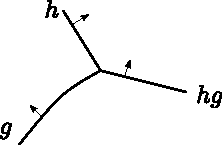
\includegraphics{junction.pdf}
\end{align}
という関係になります。

図\ref{fig:flatgaugefield}では2次元的に書いているので余次元2のジャンクションだけですが、高次元ではこのようなジャンクションがさらに集まったジャンクションもできます。3次元空間の中で泡が集まっているようなものを思い浮かべてください。

まとめると
\begin{emphasize}
  flatなゲージ場の配位は、様々な次元のトポロジカルなジャンクションを含む対称性欠陥の配位で表される。
\end{emphasize}

\subsection{Ising模型のspin flipの例}

\section{対称性欠陥のまとめ}


\section{一般化対称性}



\chapter{2次元Ising模型}

\section{2次元Ising模型と\texorpdfstring{\Ztwo}{Z2}ゲージ化}
\section{双対対称性}
\section{Kramers-Wannier 双対性}
\section{Ising模型の演算子}
\section{KW欠陥}
\section{対称性の構造}
\section{応用}


\chapter{高次形式対称性}
\section{高次形式対称性の定義}
\section{格子ゲージ理論の中心対称性}
\section{背景ゲージ場その1}
\section{背景ゲージ場その2:単体コホモロジー}
\section{自発的対称性の破れ}


\chapter{高次元の非可逆対称性}
\section{高次形式対称性のゲージ化}
\section{4次元\texorpdfstring{\Ztwo}{Z2}格子ゲージ理論}
\section{Maxwell理論}

\bibliographystyle{utphys}
\bibliography{ref}
\end{document}
